\documentclass[11pt]{article}
\usepackage[margin=1in]{geometry}
\setlength{\parindent}{0pt}
\usepackage{longtable,tabularx,multirow,vcell} 
\usepackage{mathptmx, mathtools}
\usepackage{etoolbox}
\usepackage{enumitem, esvect}
\usepackage{amsmath, amsthm, amssymb}
\usepackage{float}
\usepackage{natbib}
\usepackage[hidelinks]{hyperref}
\urlstyle{same}
\bibliographystyle{apalike}
\usepackage{blindtext}
\usepackage{fontspec}
\newfontfamily\ubuntumono{Ubuntu Mono}
\usepackage{booktabs}
\setmainfont{Times New Roman}
\newcommand\tab[1][1cm]{\hspace*{#1}}
\renewcommand{\bibsection}{}
\usepackage{caption}
\usepackage{subcaption}
\usepackage{textgreek}


\title{\textbf{Application of Godunov-Type Methods for the 1D and 2D Compressible Euler
equation*s of a Gamma Law Gas}}
\author{Wahyu Widhi Dyatmika - S421612}
\date{}

\begin{document}

\maketitle

\section{Abstract}


\section{Nomenclature}

The nomenclature of this document is shown below.
\begin{tabbing}
\textbf{Abbreviations} \= \\
\\
t \> Time [s]\\
x \> X-axis distance from datum point [m]\\
$\Phi$ \> Wave Function [Hz]\\
CFL \> Courant-Friedrichs-Lewy number [-]\\
FTCS \> Forward Time, Central Space scheme\\
u \>  Advection velocity [m/s]\\
$x_i$ \> Analytical data point\\
$y_i$ \> Numerical data point\\
$P$: \> Fraction of the program that can be parallelized\\
N: \> Maximum number of Processors
\end{tabbing}

\section{Introduction}
In this assignment, the Godunov methods are applied to one 1D problem and two 2D problems. The 1D problem consists of the Sod's shock tube problem, which is expressed by \citet{Sod1978} as follows:

\begin{equation*}
    \begin{pmatrix}
     \rho_L\\
     P_L\\
     u_L
     \end{pmatrix} =
      \begin{pmatrix}
     1.0\\
     1.0\\
     1.0
     \end{pmatrix} \cdot 
     \begin{pmatrix}
     \rho_R\\
     P_R\\
     u_R
     \end{pmatrix} =
     \begin{pmatrix}
     0.125\\
     0.1\\
     0.0
     \end{pmatrix}
\end{equation*}

On the other hand, 2D problems consists of \par
\medskip
The second problem for the 2D code is the cylindrical explosion test. This test is conducted in a domain which has a non-dimensional size of [-1:1] $\times$ [-1:1]. This domain consists of two regions, which has different properties of gas and divided by a cylinder with the radius of 0.4. The value of the gas properties are expressed as the following:
\begin{equation*}
(\rho, p) =
    \begin{cases}
        (1.0, 1.0), \ r \le 0.4 \\
        (0.125, 0.1), \ r > 0.4
    \end{cases}\!,\ u = v = 0,\ r^2 = x^2+y^2
\end{equation*}

\section{Methodology}
\subsection{Compressible Flows and Shock waves}
One of the most common compressible flow application is the treatment of discontinuities arose from the fluid properties. These discontinuities usually referred to as waves, which are commonly divided into four different types. \par
\medskip
The first type of discontinuity wave is the shockwaves, which are illustrated using the Figure \ref{fig:normalshock} below. 
\begin{figure}[ht]
    \centering
    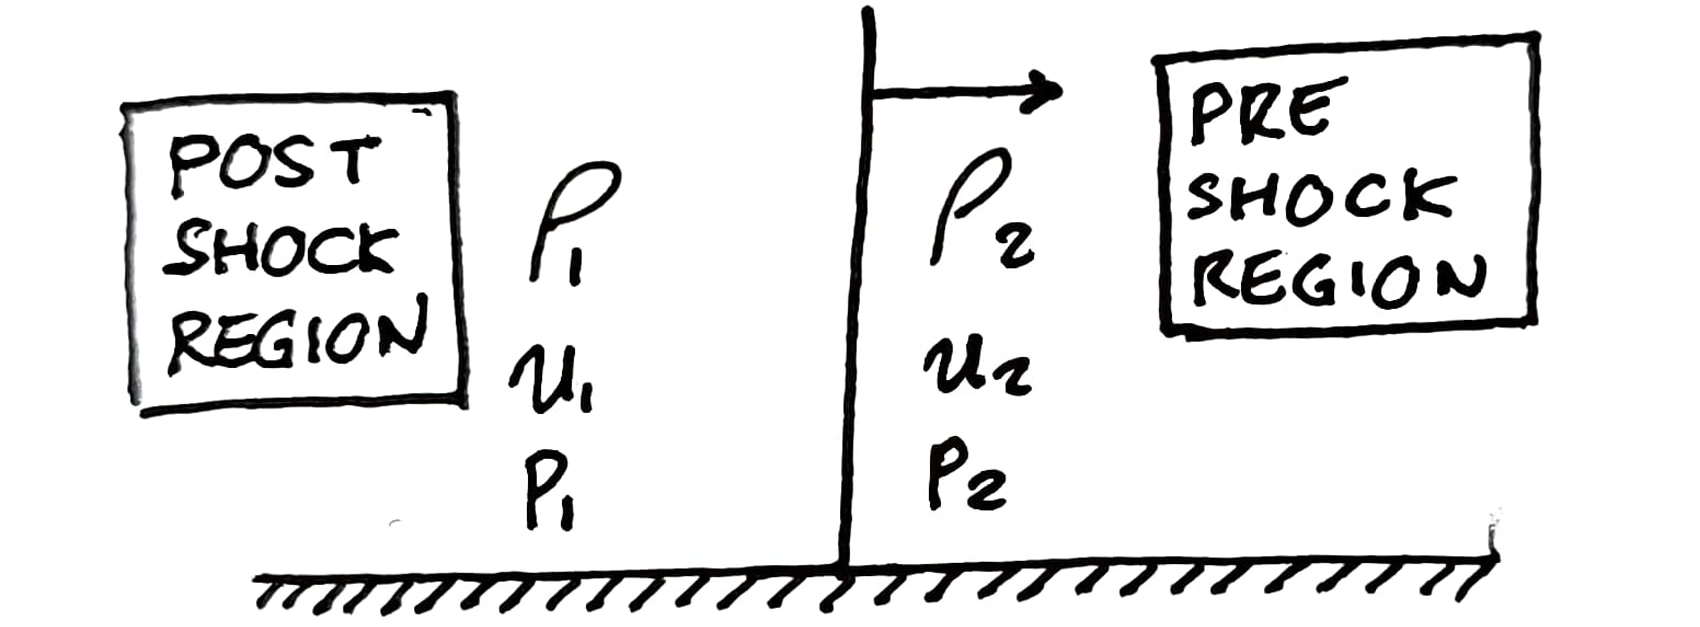
\includegraphics[width=0.4\linewidth]{Pictures/Normalshock.jpg}
    \caption{A Shockwave with Assigned Flow Property Variables (Author Illustration)}
    \label{fig:normalshock}
\end{figure}
For common shockwaves, there are several the change of properties that are present between the front and the back of the wave. The properties for the flow are:
\begin{equation*}
    \varrho_1 \ne \varrho_2 ; u_1 \ne u_2 ; P_1 \ne P_2
\end{equation*}
In this case, the properties of the wave are depended on the types of the shockwaves present in the flow. \par
\medskip
The second type of discontinuity wave is the contact discontinuity. Contact discontinuities are defined as the surfaces in which two zones with different fluid properties are met \citet{Norman1985}. The contact discontinuity is illustrated using the Figure \ref{fig:flowdisc} below.

\begin{figure}[ht]
    \centering
    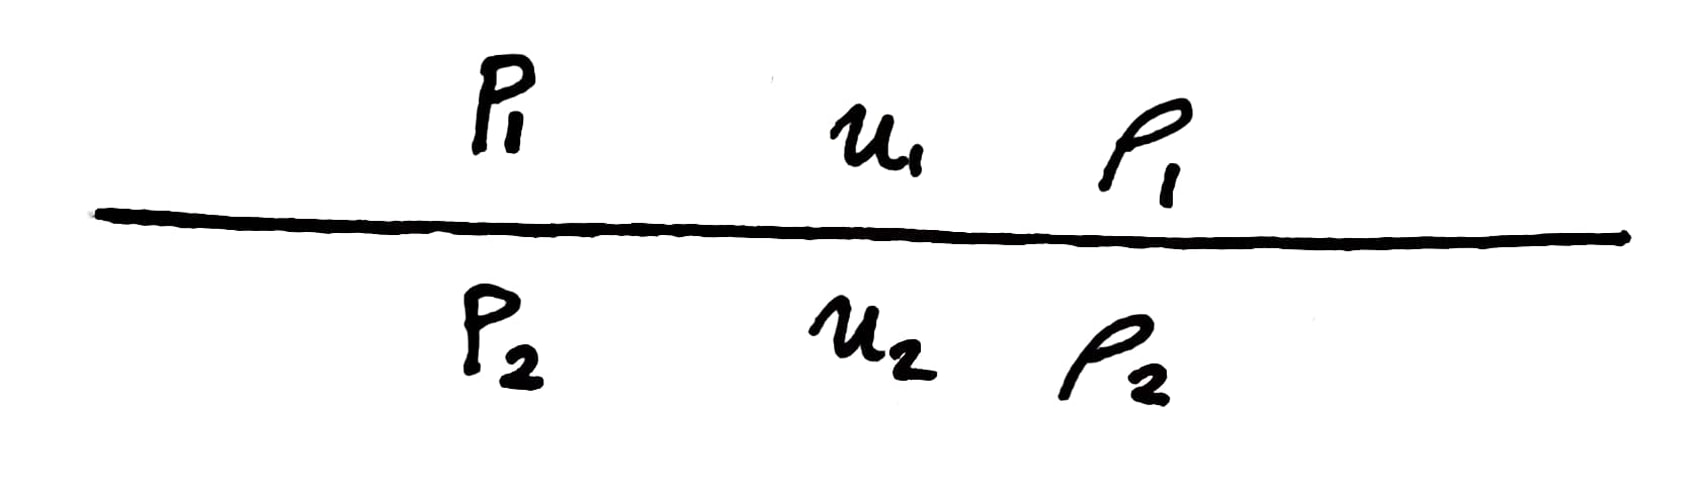
\includegraphics[width=0.4\linewidth]{Pictures/ContactDisc.jpg}
    \caption{Contact Discontinuity with Assigned Flow Property Variables}
    \label{fig:flowdisc}
\end{figure}

For the contact discontinuities, the property of the fluid flow on the two sides of the discontinuity is expressed as 
\begin{equation*}
    \varrho_1 \ne \varrho_2 ; u_1 = u_2 ; P_1 = P_2
\end{equation*}
The third type is the rarefaction or expansion wave. The flow can be defined as a discontinuity that creates lower density and pressure \citep{AMS2012}. The wave physical illustration is shown in Figure \ref{fig:rarefwave}.

\begin{figure}[ht]
    \centering
    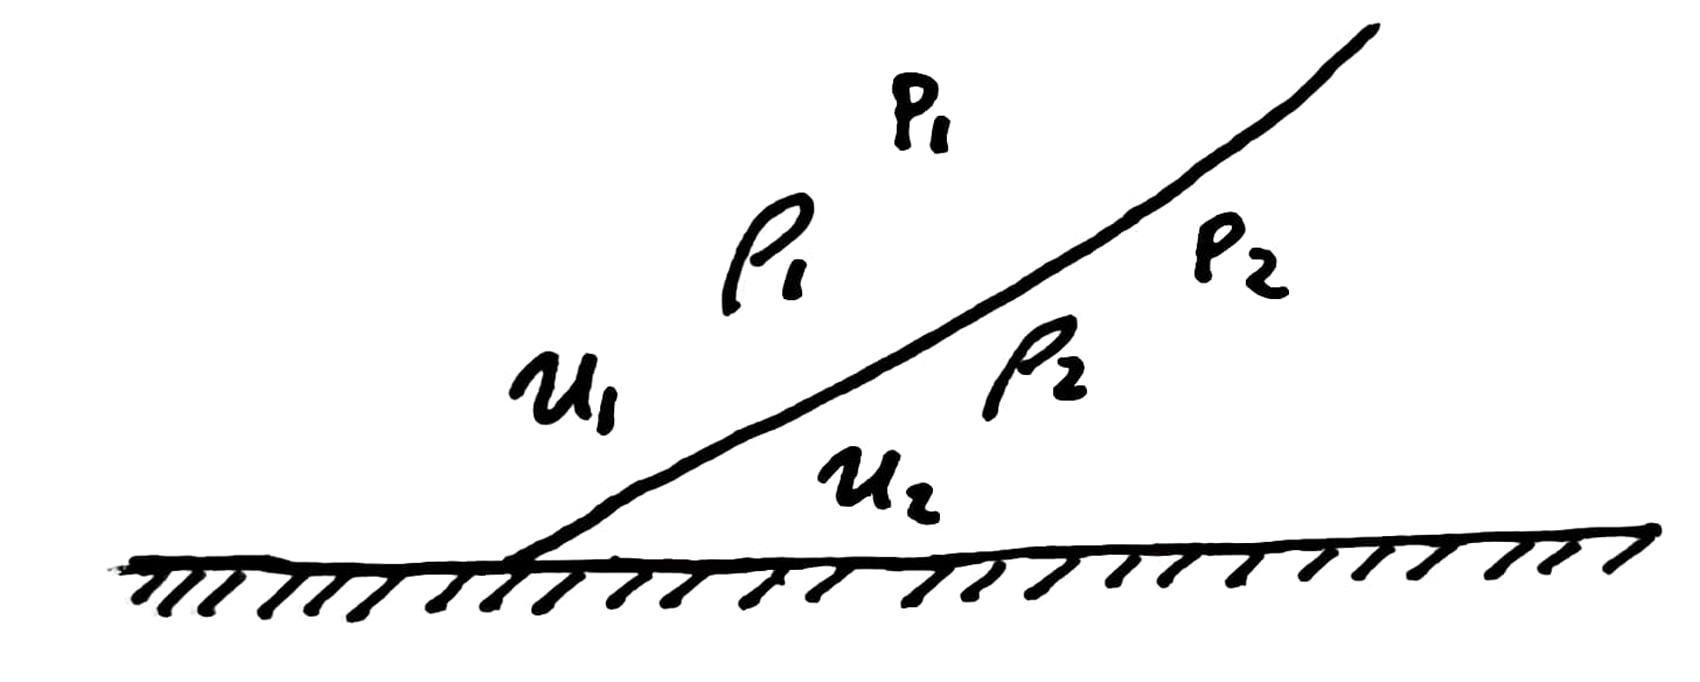
\includegraphics[width=0.4\linewidth]{Pictures/Rarefaction.jpg}
    \caption{Rarefaction Wave (Author Illustration)}
    \label{fig:rarefwave}
\end{figure}

The mathematical expressions of the value of the fluid in front and behind the wave are shown below,
\begin{equation*}
    \varrho_1 << \varrho_2 ; u_1 >> u_2 ; P_1 >> P_2
\end{equation*}

Lastly, the compression wave phenomenon creates the opposite phenomenon relative to the rarefaction wave. The flow is decelerating with increased pressure and density, expressed as below.
\begin{equation*}
    \varrho_1 >> \varrho_2 ; u_1 << u_2 ; P_1 << P_2
\end{equation*}
\subsection{Godunov method}
\label{ssc:godmethod}
Discontinuity of the flow properties commonly exists in usual compressible fluid flow analysis. To express the discontinuity, Riemann problem is used as the expression. The expression involves on using piecewise equation to understand the physics of the fluid flow \citep{Zhao2019}. \par
\medskip
In many problem cases containing discontinuity such as the compressible flow problem, the usual finite difference method is not applicable. First, finite difference method takes both of the neighbouring sides indifferently, This means that on the shock boundary, the algorithm takes the value on the pre-shock region as well as the post-shock region as the reference value \citep{Mao1992}. This creates error in the calculation as the properties at the flow are dissimilar to each other. Second, because of the treatment of primitive variables as differential equations in finite difference schemes, the equilibrium of the primitive variables is hard to maintain \citep{Zheng2021}. Third, finite difference difference method generates numerical viscosity, which smooths the discontinuity \citep{INL2024}. This creates oscillations of the results near the discontinuities and \citep{Ullrich2010}. Fourth, most of the finite difference schemes requires artificial viscosity for solving the compressible flow problem. The artificial viscosity generates additional resistance to the fluid to the shear flow to stabilise the simulation process \citep{Margolin2022}. This creates additional process to the simulation which can slow down the simulation process. Therefore, one needs to use a numerical technique that can be better at conserving the physics of the Riemann problem.\par
\medskip
Godunov methods are introduced to solve the discontinuity and preserving the concept of the Riemann problems. For 2D


\section{Results and Discussion}

\section{Conclusion}



\section{References}
\bibliography{bibliography}{}
\end{document}
